
\begin{example}
        Seja o gráfico da curva e área \ref{graf:area_para_volume} se rotacionada em torno do eixo de x forma um sólido de revolução, que tem como volume:
        \[
            S=\int_{a}^{b}\pi (f(x))^2\,dx
        \]
    \begin{figure}[ht]
  \centering
  \begin{tikzpicture}
    \begin{axis}[
      xmin=0, xmax=3,
      ymin=-0.5, ymax=2.5,
      axis x line=middle,
      axis y line=middle,
      tick align=outside,
      xtick=\empty,
      minor tick num=1,
      grid=both,
      axis line style={-{Stealth[length=3mm,width=1.5mm]}}
      ]
      % curva
      \addplot[red, thick, domain=0.5:2.5, samples=200]{0.5*(x-2)^2+1};
      \node at (0.5,-0.25) {a};  
      \node at (2.5,-0.25) {b};  
      \draw[blue, thick, dashed] (axis cs:0.5,0) -- (axis cs:0.5,2.1);
      \draw[blue, thick, dashed] (axis cs:2.5,0) -- (axis cs:2.5,1.1);
    \end{axis}
  \end{tikzpicture}
  \caption{Curva e área para volume}
  \label{graf:area_para_volume}
\end{figure}

Se for em torno do eixo de y temos:

\begin{figure}[ht]
  \centering
    \includegraphics[width=\linewidth]{Sólido_de_Revolução.png}
    \caption{Sólido gerado a partir da geratriz da figura \ref{graf:area_para_volume}}
\end{figure}

\begin{figure}[H]
  \centering
  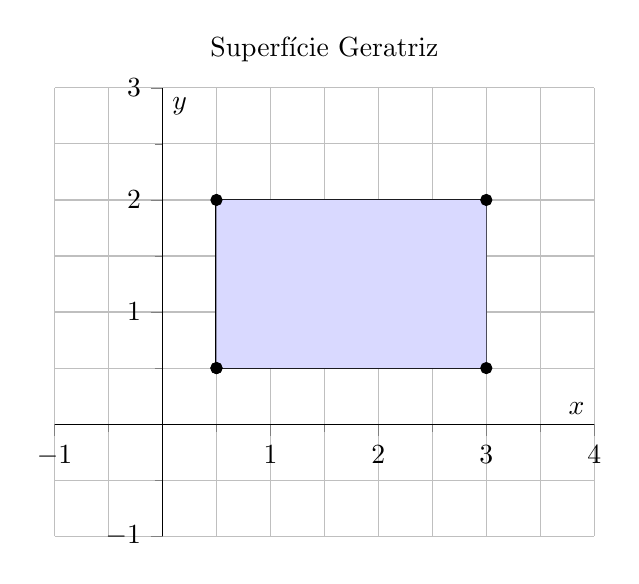
\begin{tikzpicture}
    \begin{axis}[
      xmin=-1, xmax=4,
      ymin=-1, ymax=3,
      axis x line=middle,
      axis y line=middle,
      axis line style={-},
      tick align=outside,
      grid=both,
      minor tick num=1,
      xlabel={$x$},
      ylabel={$y$},
      title={Superfície Geratriz}
    ]
      % Retângulo (fechando o caminho voltando ao primeiro ponto)
      \addplot[
        thick
      ] coordinates {
        (0.5,0.5)
        (3,0.5)
        (3,2)
        (0.5,2)
        (0.5,0.5)
      };

      % Preenchimento opcional
      \addplot[
        fill=blue!15,
        draw=none
      ] coordinates {
        (0.5,0.5)
        (3,0.5)
        (3,2)
        (0.5,2)
        (0.5,0.5)
      };

      % Pontos marcados
      \addplot[only marks, mark=*] coordinates {
        (0.5,0.5)
        (3,0.5)
        (3,2)
        (0.5,2)
        (0.5,0.5)
      };
    \end{axis}
  \end{tikzpicture}
  \caption{Superfície geratriz de um volume em torno de y}
  \label{fig:geratriz_da_superfície_y}
\end{figure}

quando a superfície é girada em torno do eixo y \ref{fig:geratriz_da_superfície_y} temos.

\begin{figure}[H]
  \centering
    \includegraphics[width=0.8\linewidth]{Cilindro_3d.png}
    \caption{Cilindro em torno de y}
\end{figure}

\end{example}